\chapter{基于知识库图嵌入的视觉问答模型}
\section{知识库概述}
人类智能体通过学习和实践不断获取知识与经验,并能将习得的知识存储在记忆系统中,面对相关问题时能准确、快速地调用相关的知识和经验,完成识别和推理过程,成功解决问题。人工智能系统的终极目标便是能像人类一般快速、准确地解决未知问题,甚至超越人类的物理极限,实现范围更广、更艰深的任务解决。人类在真实世界中的学习是不断将非结构化的信息重构为结构化的知识的过程,知识库(KB)是一种包含常识和描述真实世界的事实的知识集,在不同的应用情景中有不同的内部结构。

知识库最早被应用于人工智能中的专家系统\citing{akerkar2010knowledge},专家系统是一种建立在知识库基础上,使用推理方法完成复杂推理过程,最终实现与人类专家同水平的决策能力的计算机系统,被广泛应用于医学诊断、分子结构推理、自然语言理解等领域。专家系统面向的专家任务需要特定领域的知识,这也使得知识库成为专家系统的核心之一。针对不同领域的任务构建知识的表达方式是困难的,因为专家知识可能是不精确的,同时要从知识库中获取答案的过程依赖于人工的制定复杂的规则,知识库精度和人力成本等因素制约了专家系统在更多领域的应用。

知识库也被应用于在自然语言处理的任务,例如机器翻译和文本问答。知识库中的本体包含某个领域中的各种概念和概念间的关系,本体在机器翻译中可作为知识源\citing{nirenburg1994machine}。语言学中的多义词在不同的语境中被解释为不同的含义,人类能根据上下文语境的不同选择出最恰当的词语,但对于机器翻译系统便是一大难题。当机器翻译系统能够获得足够多的本体作为知识源时,能较好地解决多义词的解释问题,从而得到更加准确的翻译结果\citing{knight1993building}。

文本问答系统在早期作为专家系统的交互界面,在之后的发展中逐渐独立出来成为自然语言处理的一个分支,文本问答系统根据给出的文本问题,从文本知识库中提取答案,此时的文本知识库往往是文本组成的文档,还未使用资源描述框架(RDF)的结构化数据。大多数文本问答系统都采用相对标准的结构:根据问题文本建立查询、利用信息提取方法(IR)确定可能包含答案的文章位置、进一步确定答案所在的片段,这种架构下不使用任何与答案相关的额外知识\citing{hermjakob2000knowledge}。Hermjakob等人提出了将手写规则和概念本体相结合的问答系统——Webclopedia\citing{hermjakob2000knowledge}。Webclopedia由对输入问题进行句法和语义的解析的问题解析模块、用于文档查询的查询模块、用于获得与答案相关的文档的信息提取模块、片段解析模块、答案匹配模块和答案生成模块构成。系统在多个模块中使用了知识库提高精确度,在问题解析过程中使用了语言知识库——由30000个节点的概念层级、140个问题/答案类型和词库组成,帮助系统确定问题的句法结构;在查询模块中使用了WordNet\citing{miller1995wordnet}扩展与问题关键词关联的信息;在答案匹配模块中也使用了常识和事实知识库,系统的架构如图\ref{Webclopedia}。
\begin{figure}[H]
	\centering
	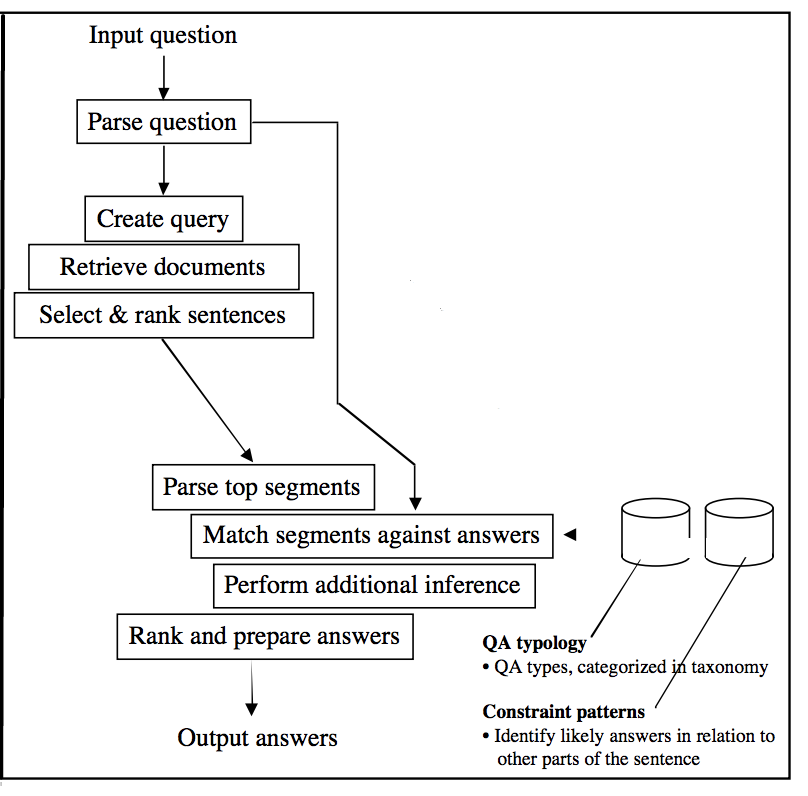
\includegraphics[width=0.8\textwidth]{Webclopedia.png}
	\caption{Webclopedia系统架构}
	\label{Webclopedia}
\end{figure}

应用信息提取技术(IR)的问答系统有一个非常明显的缺点——只能根据问题确定答案相关的文章或者段落,不能给出更为直接的答案。为解决这种缺陷,研究人员探索了更多的方法。

Burke等人一改通常的从文章中提取答案的方式,先将被频繁问到的问题(FAQ)以“问题-答案”对的形式存储为知识库,再从新问题中寻找与知识库匹配程度最高的“问题-答案”对,进而获得答案\citing{burke1997question}。在此方法中最核心的步骤是对新旧问题之间的匹配,为了使匹配的问题之间的语义相似度最大,系统还使用了WordNet\citing{miller1995wordnet}的语义知识,WordNet能提供词语和其同义词集合、同义词集合之间的关系,因此能避免一些匹配过程中的歧义错误,提高匹配的准确度。这里以“匹配”为核心思想的算法最大的障碍是常见问题集的容量、深度和广度问题,因此通常对于范围较小的场景而言,才能实现较好的匹配准确度。Rinaldi等人提出一个专门针对技术领域的基于知识的问答系统ExtrAns\citing{rinaldi2002towards}。ExtrAns以技术手册为知识库,将问题文本和知识库都转化为一种称为“最小逻辑形式”(MLF)的语义表达,并通过逻辑证明提取出答案。

随着资源描述框架(RDF)在构建知识库的兴起,知识库也由原来的文档形式转化为冗余更小、可扩展性更强、易用性更强的结构化数据库。面对由于互联网技术的普及带来的海量网页、文章、超文本、图片等多种模态的资源,研究者们对信息的整合进行了探索\citing{smith1981multibase,wiederhold1993intelligent,subrahmanian1994amalgamating,embley1998ontology,alani2003automatic},语义网和相关技术的出现促进了大尺度知识库的发展,出现了DBpedia\citing{auer2007dbpedia}、OpenIE\citing{banko2007open}、Yago\citing{suchanek2007yago}、Freebase\citing{bollacker2008freebase}、Wikidata\citing{vrandevcic2014wikidata}等多种含有常识和特定领域知识的知识库,这些配置灵活、结构统一且语义丰富的外源知识库也促进了基于知识库的视觉问答方法的兴起。

\begin{comment}
\section{常见的知识库}
知识表达是人工智能中历史较为悠久的领域,并且大量的知识表达模型被提出,从最早的“框架和脚本”(frame and script)\citing{minsky1974framework,schank2013scripts}到后来的逻辑表达方式、资源描述框架(RDF)和网络本体语言(OWL)。随着互联网技术的普及,海量的网页、文章、超文本、图片等多种模态的资源被创造,如何将这些海量松散的多模数据重组为结构化的数据成为计算机科学的重要任务之一,大量的研究对信息的整合进行了探索\citing{smith1981multibase,wiederhold1993intelligent,subrahmanian1994amalgamating,embley1998ontology,alani2003automatic},语义网和相关技术的出现促进了大尺度知识库的发展,出现了DBpedia\citing{auer2007dbpedia}、OpenIE\citing{banko2007open}、Yago\citing{suchanek2007yago}、Freebase\citing{bollacker2008freebase}、Wikidata\citing{vrandevcic2014wikidata}等多种含有常识和特定领域知识的知识库。

除了知识库以外还有一种常用的存储数据的方式——数据库。数据库通常被组织成表格的方式,表内使用数值或者字符的方式表示数据,首行罗列出不同的属性,其余行则代表存储的数据。数据库中的表与表之间存在的指针代表表之间的联系。不同于数据库,知识库不以表为组织形式,而是由大量形式为(主语,谓语,宾语)的三元组构成的图结构,这样的三元组以资源描述框架(RDF)为模型基础\citing{lassila1997resource},能够方便的通过查询语句获得信息。“主语”和“宾语”表示知识库中的实体,“谓语”代表两者之间的关系。例如,将“猫种类属于哺乳类”转化的三元组形式为(猫,种类属于,哺乳类),“猫”是主语,“种类属于”是谓语,“哺乳类”是宾语。数据库与知识库的结构对比如图\ref{db-kb}。
\begin{figure}[H]
	\centering
	\subfigure[数据库的表结构]{
		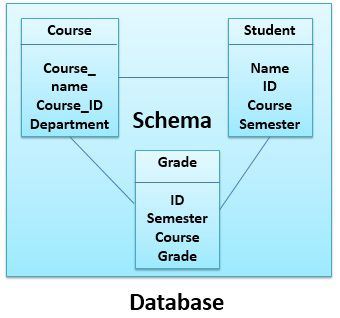
\includegraphics[width=0.5\textwidth]{database.jpg}}
	\subfigure[知识库的由三元组构成的图结构]{
		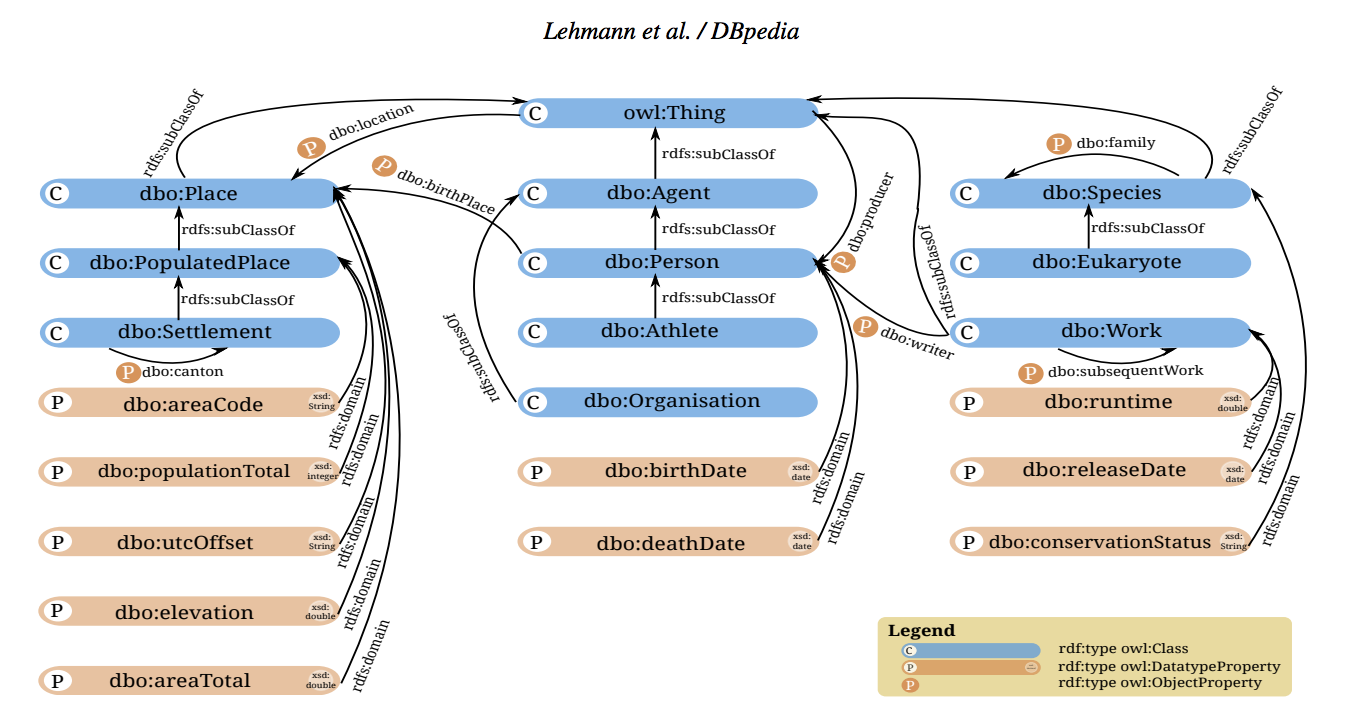
\includegraphics[width=0.7\textwidth]{kb.png}}
	\caption{数据库与知识库不同的数据组织形式}
	\label{db-kb}
\end{figure}

知识库具有高通用性、高可读性的特征。通过资源描述框架(RDF)能将所有现实中可描述的事物和事物间的关系组织到知识库中,这种通用性特征能够极大地提高了自动化系统存储、交换和使用信息;三元组的结构来源于语言学中“主谓宾”的基本语句构成方式,这既符合人类的认知方式,也是一种简单的数据组织形式,因此高可读性即使针对人类可读也是针对机器可读。正是因为知识库是建立在真实世界事实的描述之上,因此它能成为复杂决策和推理的基石,从人类推理过程看,知识库便是复杂推理的“起点”。
\end{comment}

\textbf{Yago}
知识库通常由人工和自动化提取两种方式构建得到,对比这两种不同构建方式,自动化提取的知识库往往质量较低,容易包含错误信息,而人工构建的知识库能满足较高的精度要求,但由于人工构建的成本较高,因此此类知识库有数据容量受限、构建周期长、内容老化快等缺陷。

Suchanek等人结合Wikipedia文章的广博性和WordNet优秀的语义分类,提出了自动化生成本体的知识库YAGO\citing{suchanek2007yago}。Wikipedia的文章对某个话题或概念进行详细的多角度说明,同时大多数文章都归属于一个或者多个类别,类别页面既包含了大量实体和概念,可以作为知识库中的本体,同时类别页面也隐含着概念之间的平行关系和所属关系,这能提供一定的结构关系。YAGO利用Wikipedia目录页面提取出其中的实体和实体之间的关系,同时结合WordNet中概念的清晰层次关系,实现了97\%的准确率。初始版本中涉及90万个实体和500万个实体之间的关系。

YAGO被设计为可扩展的知识库,能够结合特定领域的知识源或是从网络上提取得到的信息构建领域相关的知识库,因此之后的研究者也在此基础上进行了多种的扩展。YAGO2在YAGO基础上引入GeoNames——包含超过700万个地点信息,在“实体-关联”的表示方法中加入了时间和空间维度,不仅能丰富事实的准确性,还能反应出实体在时空层面的变化\citing{hoffart2013yago2}。YAGO3构建了一个多语言的知识库\citing{mahdisoltani2013yago3}。

\textbf{DBpedia}
Wikipedia是由非盈利组织维基媒体基金会(Wikimedia Foundation)构建的世界上最大的多语言的开放性网络百科全书,其通过文章的形式对词条进行多方面的介绍,文章中包含大量的结构化信息,例如文字、信息框模板、分类信息、图片、地理坐标信息、超链接等,这些多模态的信息能丰富知识的多样性,并且建立知识的关联。但作为网络应用,Wikipedia的搜索能力和其他网络应用一样,只能满足关键词的搜索,这种状况大大的降低了知识之间的关联和价值,同时因为其作为大规模协同性内容编辑平台,文章内容也难以避免的出现数据矛盾、不一致的分类和错误。

Auer等人为了充分挖掘Wikipedia中已有的人类知识,并构建知识结构,提出了DBpedia知识库\citing{auer2007dbpedia}。Wikipedia为实现统一的文章风格,因此在文章编辑中镶嵌了一些信息框模板,如图\ref{dbpedia}。
\begin{figure}[h]
	\centering
	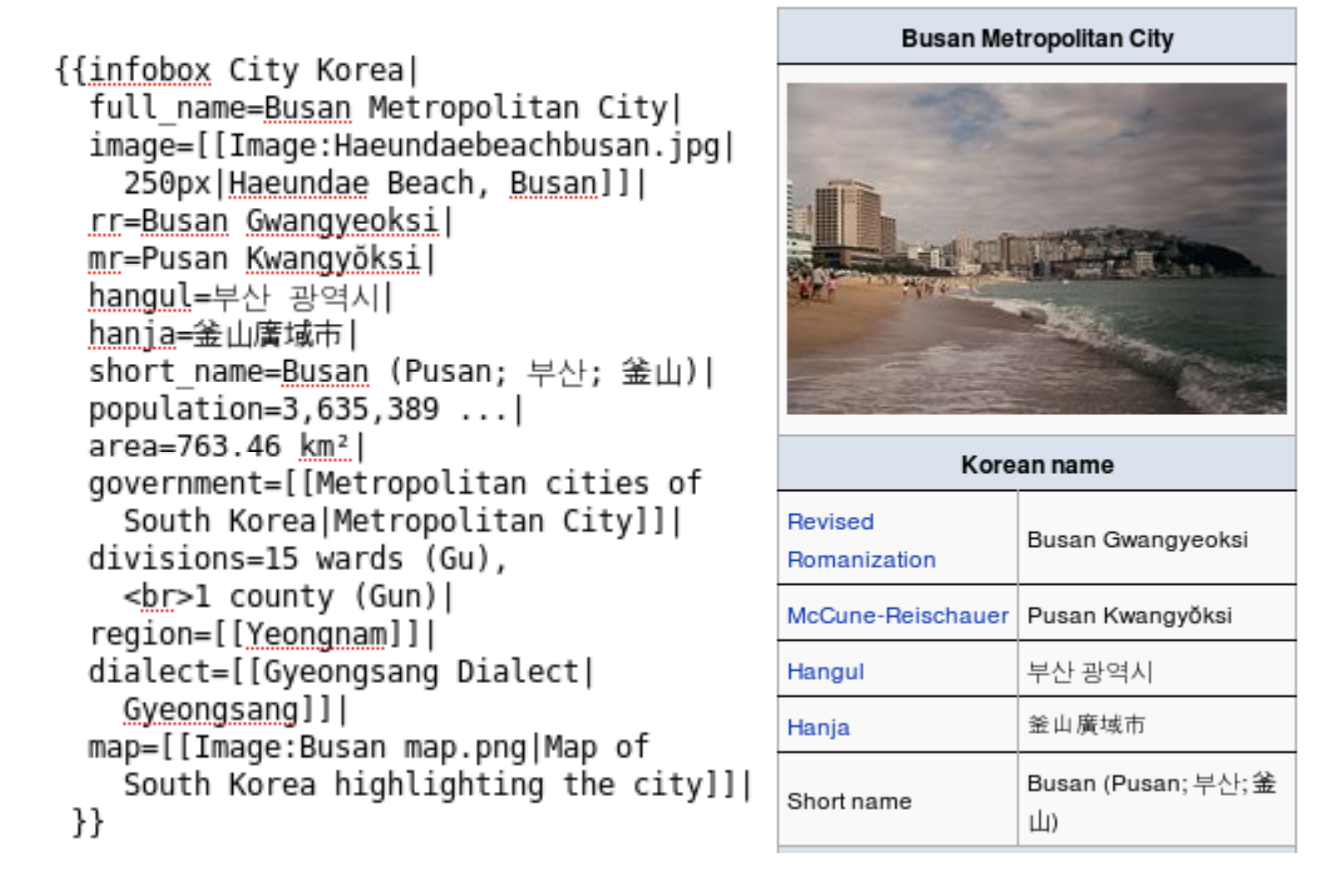
\includegraphics[width=0.8\textwidth]{dbpedia.png}
	\caption{Wikipedia的信息框模板和加载效果}
	\label{dbpedia}
\end{figure}
DBpedia利用信息框提取算法检测信息框模板,并且提取出关键的信息,再将信息转化为资源描述框架(RDF)的三元组结构,从而将Wikipedia的文章内容转化为机器可读的结构化信息。最初版本的DBpedia知识库包含关于195万实体的信息,实体内容包括人物、地点、音乐专辑和电影,除了实体外还包含65.7万个图片链接、160万个外部网页链接、18万个其他资源描述框架(RDF)数据库、20.7万个Wikipedia目录和7.5万个YAGO类别\citing{suchanek2007yago}。随着开放社区的数据丰富,2016年推出的版本中已经包含6600万实体,实体的类型扩充了视频、游戏、组织、物种和疾病\citing{wikipedia2016}。资源描述框架的三元组数据量也从1亿增长到130亿之多。

为了增强DBpedia的数据易用性,Auer等人提供了三种数据获取方式:链接数据、SPARQL协议和可下载的RDF文件。链接数据通过HTTP协议获取发布与互联网上的RDF数据,提供给语义网络浏览器、语义网路爬虫和语义网络查询客户端访问\citing{timlinked}。SPARQL是专门针对资源描述框架的查询语言,通过SPARQL终端向\url{http://dbpedia.org/sparql}发送查询指令,DBpedia知识库会返回相应的查询结果。可下载的RDF文件包含序列化的RDF三元组数据,DBpedia将整个数据库按照数据的类型分为众多子数据集,例如,文章目录集、目录标签集、地理坐标集、图像集等。

知识库的内容多样性、易用性和大体量为DBpedia应用提供了良好的基础设施,因此一些自然语言问答和交互的应用都选择建立在DBpedia丰富的知识之上。NLI-GO DBpedia是一个针对通用自然语言交互的应用程序,程序可以接受自然语言问题,并通过SPARQL查询DBpedia知识库,给出答案,实际上这就是基于DBpedia的文本问答系统\citing{nli-go},类似的还有款基于DBpedia的聊天机器人——DBpedia Chatbot。许多基于知识库的视觉问答研究也选择了数据更加准确的DBpedia\citing{wang2015explicit,wang2017fvqa,wu2016ask}。

\textbf{OpenIE}
应用于构建知识库的信息提取技术(IR)往往需要人为构建大量手写规则,并选择合适的语料库,当已有的提取模型面对全新领域的语料库时,需要重新编写提取规则或者标注数据,这种系统在面对快速迭代和具有丰富多样性的互联网数据时,便会遇到自动化程度低、语料库异质性和效率问题。

为了节省信息提取过程的自动化程度,并能大范围应用于不同领域,Banko等人提出了一种能自主学习不同语料库的信息提取模型——开放信息提取技术(Open IE)\citing{banko2007open}。Open IE以语料库为输入,通过内部算法对语料库中的语句进行一次遍历,最终提取出语句中蕴含的(实体,关系,实体)三元组数据,在整个过程中不需要人工参与,因此可以应用于不同领域知识库的构建。

Banko等人还提出了一种应用高扩展性Open IE模型的系统TEXTRUNNER。TEXTRUNNER由自监督学习器、单通道提取器、基于冗余的评估器三个主要模块构成。自监督学习器以小的语料样本作为训练集,首先使用语句解析器从样本中粗略地提取出(实体,关系,实体)的三元组数据,再对提取出的内容进行标注,标注为“可信”和“不可信”两种标签,将带有标签的数据作为朴素贝叶斯分类器的训练样本。提取器遍历整个语料库,提取出所有可能的三元组数据。对于同一个句子,提取器能生成一个或多个三元组数据,这些数据将被送入学习器训练得到的分类器中,保留所有分在“可信”类别的数据。在得到所有提取出的知识后,评估器融合相同的数据,计算不同的数据的数量。基于以上统计,评估器对每一个三元组数据分配一个用于判断知识正确性的概率值,其中的假设是,如果从多个的语句中提取出相同的知识,那么该知识拥有较高的可信度。

在实验阶段,TEXTRUNNER从包含1.3亿个句子的900万个网页中提取出6000万个三元组数据,平均每个句子提取出2.2个关系数据。通过数据过滤、随机抽取、人工判定等方式,作者对提取数据的完整性和正确性进行了概率评估,过滤后的数据包含1130万个三元组数据,其中780万的数据被评估为“格式正确”且概率标签在0.8以上,80.4\%“格式正确”的数据通过人工评估被认定为正确的,从实体间的关系看,“格式正确”的数据中反映抽象事实的占86\%,其中77.2\%是正确的;反映具体事实的占14\%,其中88.1\%是正确的,如图所示\ref{textrunner}。
\begin{figure}[H]
	\centering
	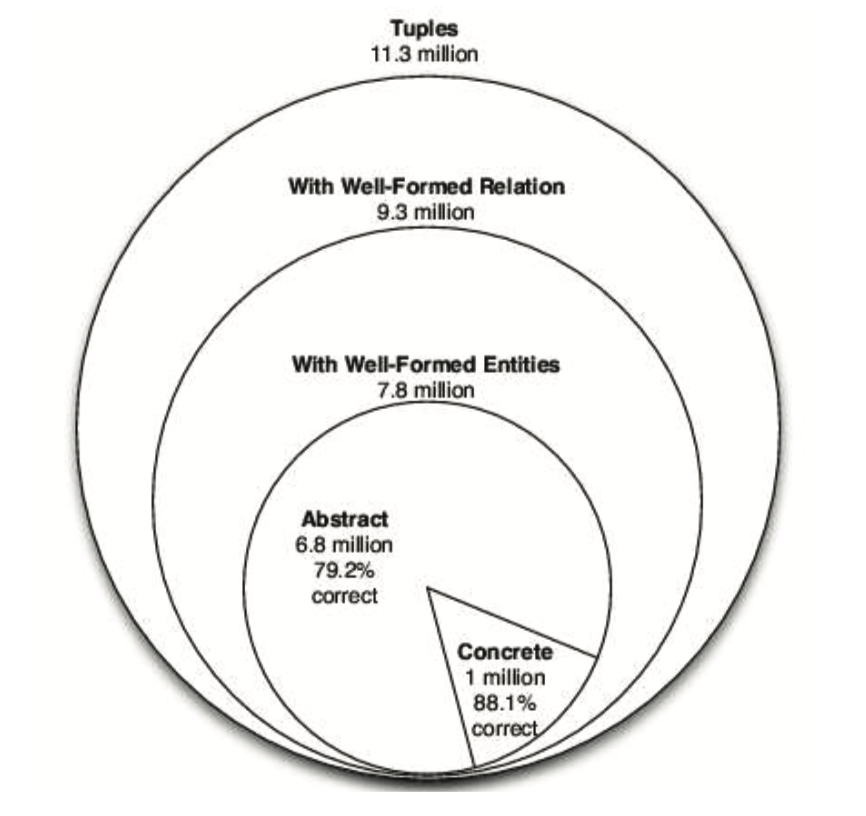
\includegraphics[width=0.5\textwidth]{textrunner.png}
	\caption{TEXTRUNNER在实验环境下知识提取的正确率}
	\label{textrunner}
\end{figure}

Wu等人在TEXTRUNNER的基础上提出了WOE开放信息提取系统\citing{wu2010open}。WOE改进了自监督学习方式用于构建提取器,TEXTRUNNER在提取过程中使用解析器直接从语料库中提取(实体,关系,实体)的三元组数据,而WOE则先从Wikipedia的信息框中提取“属性-值”对,再使用匹配器从文章中找到包含文章主语和“属性-值”对的句子作为语料库中的训练数据。随后测试了两种解析方法的提取器:WOE-parse和WOE-pos,WOE-pos使用和TEXTRUNNER类似的解析方法,根据简单的词性标签,从语料库中的句子解析出(实体,关系,实体)的数据,WOE-parse则选择更复杂的依赖解析树,希望能再复杂长句的解析中得到更好的精确度。

开放信息提取系统会对每个输出的三元组数据给定一个置信度,如果给定一个置信度的下限,高置信度的数据被保留,低置信度的数据被过滤,此时可以通过精确度和召回率测试系统的性能。精确度是指保留的数据中正确的数据所占比例,能反映整体精确度的平均水平。召回率是指保留的数据中正确的数据占所有正确数据的比例,能反映正确的数据在不同置信度的分布情况。

实验分析显示,因为使用了更友好的训练数据,WOE-pos在精确度上更优于TEXTRUNNER,而WOE-parse在解析树的帮助下实现了最好的性能,特别是在召回率上。

Fader等人在分析TEXTRUNNER和WOE的结果之后发现,不连贯提取和无信息提取两种错误频繁出现。不连贯提取是指被提取的关系语句由多词组成,但语义不连贯而无意义。无信息提取是指提取内容忽略了句子的关键信息,例如,“父亲对母亲做出承诺”,系统返回无信息的(父亲,做出,承诺)而不是(父亲,做出承诺对,母亲)。以上的两种错误都是由系统不能提取出具有完整句法结构的关系语句造成的,Fader等人在Open IE系统中引入了一定的句法限制,提出了REVERB开放信息提取系统\citing{fader2011identifying}。30\%的REVERB提取数据的概率标签在0.8或更高,相较起TEXTRUNNER的0.13\%,在精确度上实现了越阶式的增长,不连贯提取和无信息提取的错误率也大幅减少。

\textbf{Freebase}
Bollacker等人试图结合一般数据库的扩展和Wikipedia等百科全书的多样性,提出了Freebase数据库\citing{bollacker2008freebase}。Freebase和其他常用的知识库相同,使用资源描述框架的三元组形式结构化真实世界的知识,但同时继承了网络百科全书的开放和协同的思想,所有的内容创造和维护都由社区成员协作完成。Freebase存储的元组数据超过1亿2500万条,超过4000种类型和7000种属性,允许使用查询语言通过HTTP协议获取数据。

2014年,Google宣布关停Freebase并将数据迁移至Wikidata。

\textbf{Wikidata}
Wikidata是为了更高效地开放使用和管理Wikipedia文章中数据而提出的协同知识库\citing{vrandevcic2014wikidata}。由于Wikidata的出发点是希望通过大规模协同的方式构建知识库,因此Wikidata的数据具有开放性、多版本共存、多语言、易用性和持续更新的特性。Wikidata向所有用户提供数据扩展和编辑的权限;Wikidata为保证模糊数据的存疑性,相互之间有冲突的数据被同时展示;考虑到数字、日期、坐标等语言无关的数据内容,Wikidata与Wikipedia相同设计为多语言版本;Wikidata数据被组织成Json、RDF的形式发布于网络,通过网络服务能够轻松获取数据;社区成员的持续更新能保持Wikidata的时效性。

Wikidata数据的基本单元被称为项目(Item),每个项目包含名称标签、“Q+数字“的项目编码、描述、别名、和声明。声明中包含一系列属性和相应的值,用于详细描述项目的特点,项目页面如图\ref{wiki-item}。
\begin{figure}[H]
	\centering
	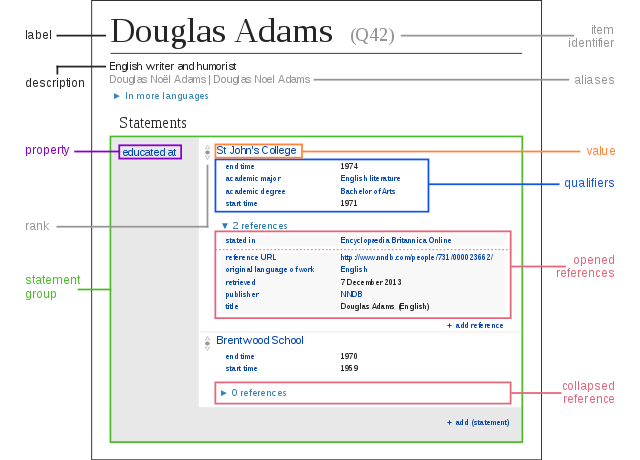
\includegraphics[width=0.8\textwidth]{wiki-item.png}
	\caption{wikidata项目页面}
	\label{wiki-item}
\end{figure}
项目之间通过有向无环图的方式构成,节点代表项目,有向线段代表项目之间的关系,如图\ref{wiki-dag}。截止到2018年,Wikidata已拥有超过5000万个项目。
\begin{figure}[H]
	\centering
	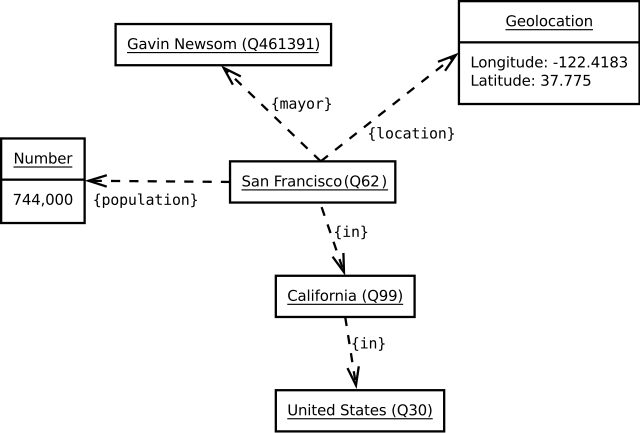
\includegraphics[width=0.8\textwidth]{wiki-dag.png}
	\caption{wikidata项目之间的有向无环图结构}
	\label{wiki-dag}
\end{figure}

Wikidata于2012年提出,相较起以往的知识库,开放性更强,限制也更少。对比YAGO和DBpedia,Wikidata不是从Wikipedia的目录或者信息框中提取信息,相反Wikidata被社区成员独立构建,并为Wikipedia作为知识源,数据被链接到Wikipedia文章中。对比Freebase将对象按类型划分的方式,Wikidata支持对所有对象赋予任意属性。

\section{KBSN模型}
使用RDF的数据表达方式,实体和实体之间通过属性建立了联系,这些有丰富语义的实体之间相互联系,构成了知识库。通过可视化的方式,实体作为节点,属性或者实体关系为边,知识库可以以图的形式呈现,因此知识库也被称为知识图谱。

正如绪论中提到的,知识库因其丰富的知识存储量、多样化的知识内容、复杂的知识关联、结构化的数据存储方式,可以作为问答系统或者其他信息检索任务的重要基础。目前使用知识图谱的主流方式是通过SPARQL等结构化查询语言对知识库中的内容进行精准的检索和提取,这种方式人为地建立查询规则、设计相应的知识库存储。

在基于知识库的视觉问答模型中,知识库的使用方式大致分为两种。一种方式为知识库查询类,依照主流的知识库查询的思路,模型提取图片的实体、将实体映射到知识库、转化自然语言为查询语句、查询知识库\citing{wang2015explicit, wang2017fvqa}。这些模型依靠精准的查询语句,对于预先设定好的模板问题能实现优于基线模型的准确率,然而却面临着问题模板设计成本高、数据集难构建、模型泛化能力差等缺点。

另一种方式为联合嵌入类,这种方式不用设计复杂的查询语句,而是将知识库的文本信息转化为额外的特征向量,并联合图像特征和问题特征一起训练。这种方式能省去问题模板和查询语句设计的人工成本,并将模型在更大规模的开放性数据集进行训练。然而,此前的模型却仅仅使用知识库中单个节点的文本信息,例如论文\citing{wu2016ask}根据从图像中预测的属性生成DBpedia查询,得到相关属性的“comment”本文内容,再将这种成段的文本信息转换为固定的特征向量,作为由知识库提供的额外特征与其他两种模态的特征融合。在这种方式中,模型虽然引入了额外的特征,试图提高表征能力,但是这种额外特征仅仅局限于单个节点,因此必然损失了节点互联形成的结构关系,而这种结构关系正是知识库的核心——通过多种关系连接而组织起来的具有丰富语义表征能力的实体网络。

为了利用知识库中关联数据的结构信息,我们在N-KBSN模型的基础上,引入使用图嵌入表示的知识库,提出了KBSN模型。KBSN模型使用了N-KBSN模型的问题文本和图像特征提取模块、自注意力和引导注意力模块,而在特征融合时引入了知识库的图嵌入。

知识库的图嵌入是KBSN模型有别于其他基于知识库的视觉问答模型的创新之处,其背后的思路为:先从图像和问题文本中识别出核心概念,将核心概念映射为知识库中的核心实体,通过剔除核心实体外无关的实体和链接形成以核心实体为中心的子图,再将各个子图转换为图嵌入,最后子图嵌入融合为图嵌入,以此作为额外特征。

按照以上的思路,知识库的图嵌入由子图提取模块和子图嵌入模块两个主要部分组成。子图提取模块的作用是完成从图像和问题文本到知识库的映射。具体来说,子图提取模块包含“图像-知识库映射”和“文本-知识库映射”。“图像-知识库映射”使用Faster R-CNN预测得到图像中包含的物体,再使用SPARQL查询知识库,得到图像相关的核心实体,“文本-知识库映射”使用DBpedia Spotlight\citing{isem2013daiber}模型识别、整合问题文本,得到问题相关的核心实体。需要指出的是,在此,我们不是使用完整的DBpedia知识库,而是根据问答这种任务类型的特点,挑选出特定的数据子集构成实验知识库。

子图嵌入模块是将提取得到的子图映射为图嵌入。具体来说,我们首先使用实验知识库训练TransE模型,得到实验知识库的嵌入表示。然而将子图提取模块输出的子图的节点和边都映射为向量,最后经过图神经网络获得子图的嵌入表示。

最后将子图的嵌入表示、图像特征、文本特征三者融合,分类得到答案,KBSN的基础架构如图\ref{KBSN}。
\begin{figure}[H]
	\centering
	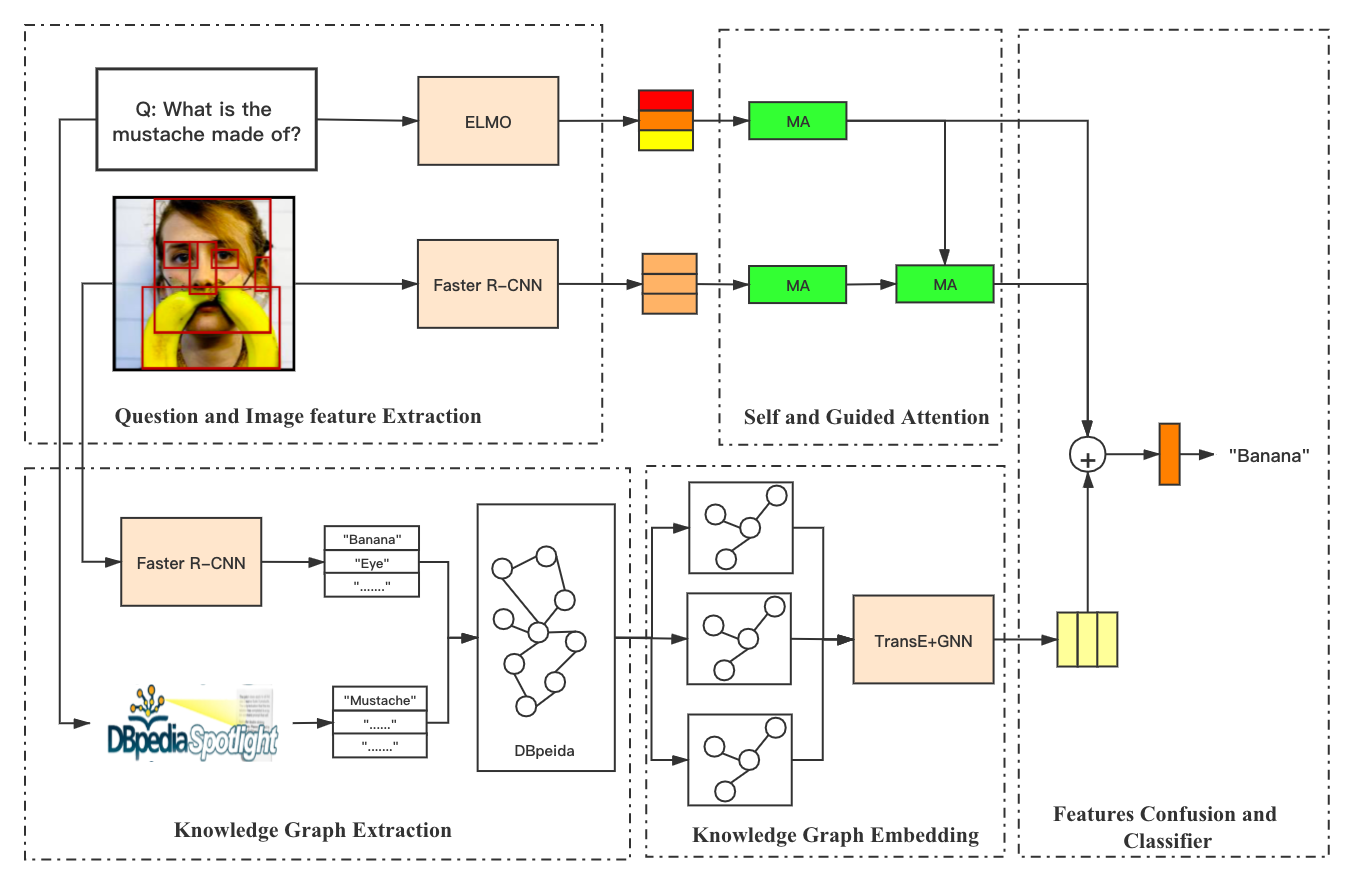
\includegraphics[width=0.8\textwidth]{KBSN.png}
	\caption{KBSN的基础架构}
	\label{KBSN}
\end{figure}

\subsection{知识库子图提取}
对于基于知识库的视觉问答任务而言,准确的实现自然语言和图像中涉及的实体到知识库实体的映射是至关重要的,一方面能够大大地减少知识库中无关信息的噪声干扰,提高精确度,另一方面准确的映射能够极大的减少计算冗余,提高运行速度。

在知识库子图提取的准确性和计算效率综合的考量下,我们首先以DBpedia为基础,收集了部分子数据集组成实验知识库,再使用在N-KBSN模型中相同的Faster R-CNN从图像中识别出关键实体,再设计SPARQL查询语句从实验知识库中提取出图像相关的子图。另一方面,对于问题文本中的核心实体,我们直接使用DBpedia Spotlight完成从文本到DBpedia节点的映射,进而提取出问题相关的子图。

需要注意的是,针对图像的物体识别是使用的N-KBSN的Faster R-CNN,但是在N-KBSN中,是将所有区域的图像特征融合作为图像特征,而此处则加上分类层,使用softmax预测并输出各个区域的类别信息。由于使用的Faster R-CNN已经在之前的章节详细介绍了,本节将省略面向图像的子图提取,重点介绍面向文本的子图提取。

\subsubsection{知识库收集和分析}
在本文中,因为DBpedia丰富的实体及其属性,并且相对规范和统一的数据内容,我们使用DBpedia作为提供额外特征的知识库。然而由于DBpedia从众包的wikipedia提取得到,因此知识库中除去我们关心的和实体语义高度相关的属性外,还保留着一些基于语义网思想的属性,例如用于连接其他知识库实体的外链、参考引用的外链、主页地址、图片链接、未经处理的infobox属性等,除此之外,完整数据集中还包含包括英语在内的多语言版本,而以上这些信息对于回答开放性问题帮助很小,因此在本文的研究中,我们甄选了DBpedia数据集中“语义高度相关”的子数据集构成实验知识库,具体的数据集和其简要描述如表\ref{dbpeidaList},知识库的参数统计如表\ref{dbpediaPara}。
\begin{table}[H]
% \resizebox{0.8\textwidth}{!}{}
\centering
\caption{实验知识库包含的DBpedia数据子集及其描述}
\begin{tabular*}{0.9\textwidth}{lc}
\toprule
\textbf{DBpedia数据集} & \textbf{描述}\\
\midrule
instance\_types\_en & 连接实体及其类型 \\
labels\_en & 实体标签 \\
mappingbased\_literals\_en & 连接object为literal的高质量的谓语 \\
mappingbased\_objects\_en & 连接object为对象的高质量的谓语 \\
persondata\_en & 和person相关的信息,例如出生日期等 \\
\bottomrule
\end{tabular*}
\label{dbpeidaList}
\end{table}
\begin{table}[H]
% \resizebox{0.8\textwidth}{!}{}
\centering
\caption{实验知识库的参数统计}
\begin{tabular}{lc}
\toprule
\textbf{统计参数} & \textbf{数量}\\
\midrule
三元组 &  59,998,758\\
类 &  426\\
实体 & 5,377,081 \\
主语 & 14,556,042 \\
属性 & 1,377 \\
宾语 & 19,495,719 \\
\bottomrule
\end{tabular}
\label{dbpediaPara}
\end{table}

正如表\ref{dbpeidaList}所示,实验知识库只包含了英语版本的知识库,但值得注意的是,本文提出的模型结构同样适用于其他语言类型,扩展到多语言的应用只需要将数据集和知识库替换为指定语言版本即可。实验知识库包含完整的类别信息、完整的实体标签和高质量的属性信息,足够应对绝大部分的常规问题,例如VQA2.0数据集中涉及的对象和属性都存在于实验知识库中。

我们使用virtuoso opensource将上述数据集加载成一个命名图(http://dbpedia.org),并使用本地服务器提供SPARQL应用交互接口,以便后续提取子图。

\subsubsection{面向文本的子图提取}
和基于知识库的问答任务相似,基于知识库的视觉问答任务中的问题文本中并不是每个词语对于答案的得出都起着同等重要的作用。例如对于问题“Is this book writen by Ernest Miller Hemingway”,人类回答者可以忽略句式中的谓语"is"、代词"this",而将句子缩减为(book, writen by, Ernest Miller Hemingway)。这种去除了辅助句法和语法结构的词语而得到的缩减形式便能够反映问题的关键信息,而其中的"book"和"Ernest Miller Hemingway"这类名词在知识库中,被称之为命名实体(named entity),在DBpedia中是以类似于$DBpedia:book$和$DBpedia:Ernest\_Miller\_Hemingway$这种URI的节点形式存在。

对于这些存在于文本中的命名实体的提取便是本小节中面向文本的子图提取的关键步骤之一。而在命名实体的提取中,消除歧义是非常重要的。同一个单词在不同的语境下表达不同的意思,如果不能根据语境正确地判断出单词的特定语义,那么句义的理解就可能偏移,甚至意思完全无法理解。在文本-知识库映射中则体现为,同一个单词子不同语境下对应不同的DBpedia资源,例如"Washington"可以同时对应$DBpedia:George\_Washington$和$DBpedia:Washington,\_D.C$,前者指向“乔治-华盛顿”,一个人,而后者则指向“华盛顿特区”,一个地方,两者的含义千差万别。

为了实现较为准确的命名实体识别,我们使用DBpedia Spotlight模型\citing{mendes2011dbpedia}实现文本-知识库映射。包括“人物”、“地点”、“组织”这种常见的类别,DBpedia Spotlight能够实现272类DBpedia资源的识别,因此能够很好的识别绝大部分问题中涉及的实体。我们还可以通过针对数据集的特点使用针对性的配置,进一步提高实体的识别准确率。

DBpedia Spotlight模型主要由三个阶段实现,短语识别阶段从输入的自然语言句子中提取出可能存在DBpedia资源的短语;候选实体筛选阶段将前一阶段得到的一系列短语映射到DBpedia资源,形成候选实体列表;消除歧义阶段根据短语的上下文语境,从候选实体列表中挑选出最佳的DBpedia资源,完成从文本-知识库映射。

短语识别阶段首先通过字符匹配算法从句子中提取词典中包含的短语,再对每个短语自动标注词性,并且去除词性为动词、形容词、副词、介词,剩下的短语作为候选短语。

候选实体筛选阶段根据DBpedia的Disambiguation数据集——包含和特定短语容易混淆的所有其他短语,囊括每一个候选短语的歧义形式的DBpedia资源,例如对于候选短语"Washington",$DBpedia:George\_Washington$和$DBpedia:Washington,\_D.C$都被加入候选实体列表,以便下一阶段的使用。这一阶段实现了由短语到DBpedia资源的映射,并且为了提高结果的准确性,在这一阶段只进行最小化的筛选,尽量多的包含候选实体。

消除歧义阶段使用生成概率模型\citing{han2011generative},根据短语的上下文信息,计算短语和实体匹配的概率,再依照概率阈值得到短语匹配的DBpedia资源,其中短语也称为“实体指称”。假定短语$s$,上下文$c$,每个实体$e$和短语匹配的概率可以根据以下公式得到,
\begin{equation}
P(e,s,c) = P(e)P(s|e)P(c|e)
\end{equation}
其中,$P(e)$表示实体出现的概率,$P(s|e)$表示以短语$s$指代实体$e$的概率,因为多种不同的短语可以指代同一个DBpedia资源,例如短语"Washington"和"George\_Washington"都可以指代$DBpedia:George\_Washington$,$P(c|e)$表示实体在特定语境出现的概率。通过最大似然概率,得到最匹配的实体$e$,即
\begin{equation}
e = argmaxP(e,s,c)
\end{equation}

假定一个包含$M$个实体指称的wikipedia数据集,$P(e)$可以使用以下公式计算,
\begin{equation}
P(e) = \frac{count(e)}{|M|}
\end{equation}
其中$count(e)$表示指向实体$e$的实体指称的数量。$P(s|e)$的公式为,
\begin{equation}
P(s|e) = \frac{count(e,s)}{count(e)}
\end{equation}

对于短语$s$,它的上下文$c$可以使用一个单词窗口来框定,在本文中,我们设定窗口大小为50。假定上下文$c$包含$n$个单词$t_1t_2...t_n$,那么$P(c|e)$的公式为,
\begin{equation}
P(c|e) = P_e(t_1)P_e(t_2)...P_e(t_n)
\end{equation}
其中$P_e(t)$表示单词$t$出现在实体$e$的上下文的概率,计算公式为,
\begin{equation}
P_e(t) = \lambda P_{e-ML}(t) + (1-\lambda)P_{LM}(t)
\end{equation}
\begin{equation}
P_{e-ML}(t) = \frac{count_e(t)}{\sum_t count_e(t)}
\end{equation}
其中$P_{e-ML}(t)$是$P_e(t)$的最大概率,$P_{LM}(t)$是在wikipedia数据集上计算得到的通用语言模型。

为了防止短语都连接到“空实体”,同样我们需要计算“空实体”的得分$P(NIL,s,c)$,使用以下公式分别计算$P(NIL)$、$P(s|NIL)$和$P(c|NIL)$,
\begin{equation}
P(NIL) = \frac{1}{|M|}
\end{equation}
\begin{equation}
P(s|NIL) = \prod_{t\in S}P_{LM}(t)
\end{equation}
\begin{equation}
P(c|NIL) = \prod_{t\in C}P_{LM}(t)
\end{equation}
而所有得分小于$P(NIL,s,c)$的实体都会被剔除。

在计算得到实体的得分之后,根据得分的高低排序便可以得到最匹配的DBpedia资源,完成文本-知识库映射。

%\subsubsection{面向图像的子图提取}

\subsection{知识库子图嵌入}
针对本文提出的KBSN模型,我们将从问题文本中提取得到的DBpedia实体视为核心节点,核心节点从词性的角度看,绝大多数都为名词,从句义的整体来看代表整个句子的核心概念,例如问题“Is there snow on the mountains?”中,我们提取出实体$DBpedia:Snow$,并且提取出以Snow为核心节点的子图。子图中包含大量语义高度相关的属性能作为丰富概念的不同语义层次,例如其属性Subject为$Category:Snow$——表示其分类,属性seeAlso为Blizzard——表示其同义概念。然而图结构的知识子图并不能很好的计算处理,因此我们使用分布式表示将知识子图中的实体和关系转化为低维向量。这样做的优点有以下几点:
\begin{itemize}
  \item [1)] 
  计算的便利性,向量化的节点能够方便的衡量节点的差异和相似度,显著提升计算效率。 
  \item [2)]
  实现多模信息的融合,KBSN模型中涉及图像特征、文本特征和知识子图特征三种不同模态的数据结构。知识子图的嵌入能够很好得融合入另外两种特征,这种统一的特征表达方式能够也是适应目前的计算框架——以多维向量为基础的计算方式。
  \item [3)]
  便于知识库的扩展,文本使用DBpedia为主要的知识库,然而对于其他主流的知识库,如Freebase,WordNet等,使用的实体和属性名称不尽相同,这会限制模型迁移。而使用分布式表示能够将不同的知识来源映射到同一个语义空间,从而建立统一的表示空间,实现不同知识库的相互适应,提高模型的扩展能力。
\end{itemize}

文本将使用TransE\citing{bordes2013translating}模型为基础,实现对子图的嵌入表示。TransE模型的思路来源于词向量中呈现出的词向量聚集和向量空间的平移不变性。具体来说,在词嵌入空间中具有相似语义的词表示呈现出聚集情况,例如向量$e(German)$和$e(France)$等国家名称距离接近;平移不变性表现为$e(king)-e(queen)\approx e(man)-e(woman)$。前者说明有效的嵌入能够表征词的语义相似性,后者说明向量空间中存在一些固定关系能够连接不同的词嵌入。而在知识库中实体之间是通过显性的关系连接构成一个三元组,这种显性的关系也许能帮助找到一个好的图嵌入方式,使得向量空间中存在和显性关系暗合的隐藏关系,而这种隐藏关系在TransE中被称为“翻译”。假定E为实体的集合,R为关系的集合,训练集为$S=\{(h,r,t)\}$,其中三元组(h,r,t)中h表示“头实体”,r表示“关系”,t表示“尾实体”,它们的嵌入向量分别用$l_h$、$l_r$、$l_t$表示。TransE希望得到的向量存在以下关系,
\begin{equation}
l_h+l_r \approx l_t
\end{equation}
公式可以看做向量$l_h$经过关系r翻译后得到了$l_t$。

为了学习到符合以上公式的向量,模型使用$d(h+r, t)$计算两个向量的差异度,函数d使用L1或者L2距离计算公式。模型的思路为如果对一个正确存在的三元组的h或者t替换成其他的实体,那么新的差异度$d(h^n,r,t^n)$数值应该尽量大,以体现新三元组的错误性。因此TransE使用以下损失函数,
\begin{equation}
Loss = \sum_{(h,r,t) \in S}\sum_{(h^n,r,t^n)\in S^n}|\gamma+d(h+r, t)-d(h^n,r,t^n)|
\end{equation}

其中,$\gamma$为正确的三元组和错误三元组差异度之间的距离超参数。
\begin{equation}
S^n = {(h^n,r,t)|h^n \in E} \cup {(h^n,l,t)|t^n \in E}
\end{equation}
$S^n$表示替换了头实体或者尾实体的三元组的集合。

比起以往的模型,TransE参数较少,计算复杂度低,但能够直接建立实体和关系的复杂语义联系,并且在大规模的知识库上依然有较好的表现,因此文本将使用TransE将知识库子图中的实体和关系转化为向量表示。

本文TransE的参数设置为,向量维度$k=50$,随机梯度下降的学习率$\lambda=0.0.1$,$\gamma=1$,$d()$使用L2距离公式。

\subsection{基于图神经网络的图嵌入}
现实中存在大量可以被转化为图结构的数据,例如化学分子结构、交通网络、知识关联甚至图像,从图结构中挖掘数据关联是图的研究的一个重要领域。在图神经网络被提出以前,传统机器学习处理图的方式主要是通过将图结构转化成形式更简单的数据形式,例如向量\citing{haykin2004comprehensive}。这种图结构简单化的压缩方式损失了图的拓扑结构信息——压缩后的向量不含有节点之间的连接关系,因此缺乏表征能力。为了解决这一问题,Scarselli等人提出了图神经网络(GNN)\citing{scarselli2008graph}。受循环神经网络和马尔科夫链在图结构数据上的应用,GNN统一了两者的优势,使用信息传递机制,不断更新一系列对应图节点的单元,直到节点状态达到稳定的平衡,最后基于这些节点输出结果。由于这种架构能够处理更为广泛的图,例如有向图、无向图、有环图、无环图,成为了近年来新兴的基于统计的图研究方法。

受到卷积网络在计算机视觉领域所获巨大成功的激励,近来出现了很多为图数据重新定义卷积概念的方法。这些方法属于图卷积网络(GCN)的范畴。Bruna\citing{bruna2013spectral}等人于2013年提出了关于图卷积网络的第一项重要研究,他们基于谱图论(spectral graph theory)开发了一种图卷积的变体,这种方法直接使用图的拓扑结构,根据图的邻居信息进行信息收集。但是由于基于频谱的模型的计算成本随着图的大小而急剧增加,因此对于大图的计算效率较低,另外这种模型只能使用静态的图,面对动态更新的图时,需要执行全新的计算,因此模型的适应性不好。而基于空间的图卷积网络可以解决上述问题,因此也成为了现在主流的GCN方法。这些方法遵循循环递归邻域聚合(或者消息传递)的模式
,其中每个节点聚合其相邻节点的特征向量用于更新当前节点的特征向量,在多轮聚合迭代后,这种聚合了邻居节点信息的特征向量被用来表示该节点。再根据任务的需要决定输出节点层级的特征(node-level)或者图层级的特征(graph-level)。

在一般的图中,节点可以表示不同的实体,但是连接节点的边没有区别,都只表示为一种连接关系。然而,知识图谱的边具有语义信息,表示实体之间的特定关系,且不同的边可能具有巨大差异的语义,因此除了节点需要表征为向量,边也需要。假设$G = (V, E)$表示一个图,$X(v_i)$表示节点$i$的节点向量,$v_i \in V $,$X(e_{i,j})$表示节点$v_i, v_j$之间的边向量,$e_{i,j} \in E$。GNN 利用图结构和节点特征 $X(v_i)$ 来学习一个节点的表征向量 $h(v_i)$,或者整个图的表征向量 $h(G)$。遵循领域聚合策略,我们通过聚合它的邻近节点的表征向量来迭代更新节点的表征向量,在第$k$层,
\begin{equation}
a_{v_i}^{(k)} = AGGREGATE^{(k)}(Tr(h_{e_j}^{(k-1)}, X(e_{i,j}))), v_j \in N(v_i)
\end{equation}
其中$v_j$为节点$v_i$的邻接节点,$Tr(h_{e_j}^{(k-1)}, X(e_{i,j}))$将上一层的节点的表征向量联合边向量进行融合,$AGGREGATE()$为该层的聚合向量。而$k$层的节点表征向量由下式得到,
\begin{equation}
h_{v_i}^{(k)} = COMBINE(h_{v_i}^{(k-1)}, a_{v_i}^{(k)})
\end{equation}
其中,我们初始化$h_{v_i}^{(0)}=X(v_i)$。

不同的$AGGREGATE{k}() $和 $COMBINE{k}() $能组合出不同的用于聚合的体系结构,在本文中,我们使用GCN\citing{kipf2016semi}中的方式,将AGGREGATE 和 COMBINE 步集成在一体如下:
\begin{equation}
h_{v_i}^{(k)} = ReLU(W*MEAN\{Tr(h_{v_j}^{(k-1)}, X(e_{i,j})), h_{v_i}^{(k-1)}\}), v_j \in N(v_i)
\end{equation}
其中$MEAN\{\}$为element-wise的均值池化。

并且为了让知识库中的节点向量能和文本处理模块保持语义的一致性,我们使用elmo初始化节点和边特征,即,
\begin{equation}
X(v_i) = elmo(v_i),
X(e_{i,j}) = elmo(e_{i,j})
\end{equation}

\section{实验}
\subsection{数据集}
\subsection{实验结果分析}

\section{本章小结}

